\section{Charge Transfer Properties}
We have seen that the final structure of the pentacene systems becomes more ordered and crystal-like as the quenching time is increased. It would be good now to see how this affects the charge transfer properties. A key quantity governing charge transfer rates is the ratio between electronic coupling and reorganisation energy, $\frac{H_{ab}}{\lambda}$. Seeing as we have a single molecule system, by plotting the electronic coupling we can get a qualitative view of the charge transfer dynamics and see which paths are the most likely within the structure.
\subsection{Global Couplings}
\begin{figure}[ht]
	\includegraphics[width=\textwidth]{./img/DifferentQuenchTimes/GlobalCouplings.png}
	\caption{\label{fig:glob_coup}The global coupling distribution for each of the quenched structures (in blue, orange, green and red) and 1 structure after a 10ns quench without using electrostatics (purple line). The black dashed lines represent the maximum coupling within a perfect pentacene crystal.}
\end{figure}
\noindent The global coupling distribution gives an overview of the values of coupling within the system, hence an idea of the charge transport properties of the system. To calculate these couplings I have used the analytic overlap method (AOM)\cite{gajdos_ultrafast_2014} between all pairs of molecules (using a nearest neighbour cutoff) in the final snapshot of each quenched system. As can be seen from figure \ref{fig:glob_coup}, as the quench time increases a knee starts to form in the distribution at a high coupling value ($~80 meV$). This is especially obvious in the 100ns quench structure (red curve) which has far fewer lower energy couplings and more coupling values approaching the crystal maximum of $117$meV.
\\\\
The figure also highlights the importance of a correct account of electrostatic interactions in the formation of these structures. The purple line shows the coupling distribution for the same simulation without any electrostatics. In this curve we see far more very high values of coupling -substantially higher than those seen in the perfect crystal. This is due to it now being energetically favourable to form a more tightly packed face-to-face structures giving rise to larger molecular overlaps hence higher couplings. We see all the other distributions fit well between the 2 black lines, which denote the maximum coupling value in a perfect crystal.
\subsection{Coupling Networks}
\label{sect:couplGraphs}
\begin{figure}[ht]
	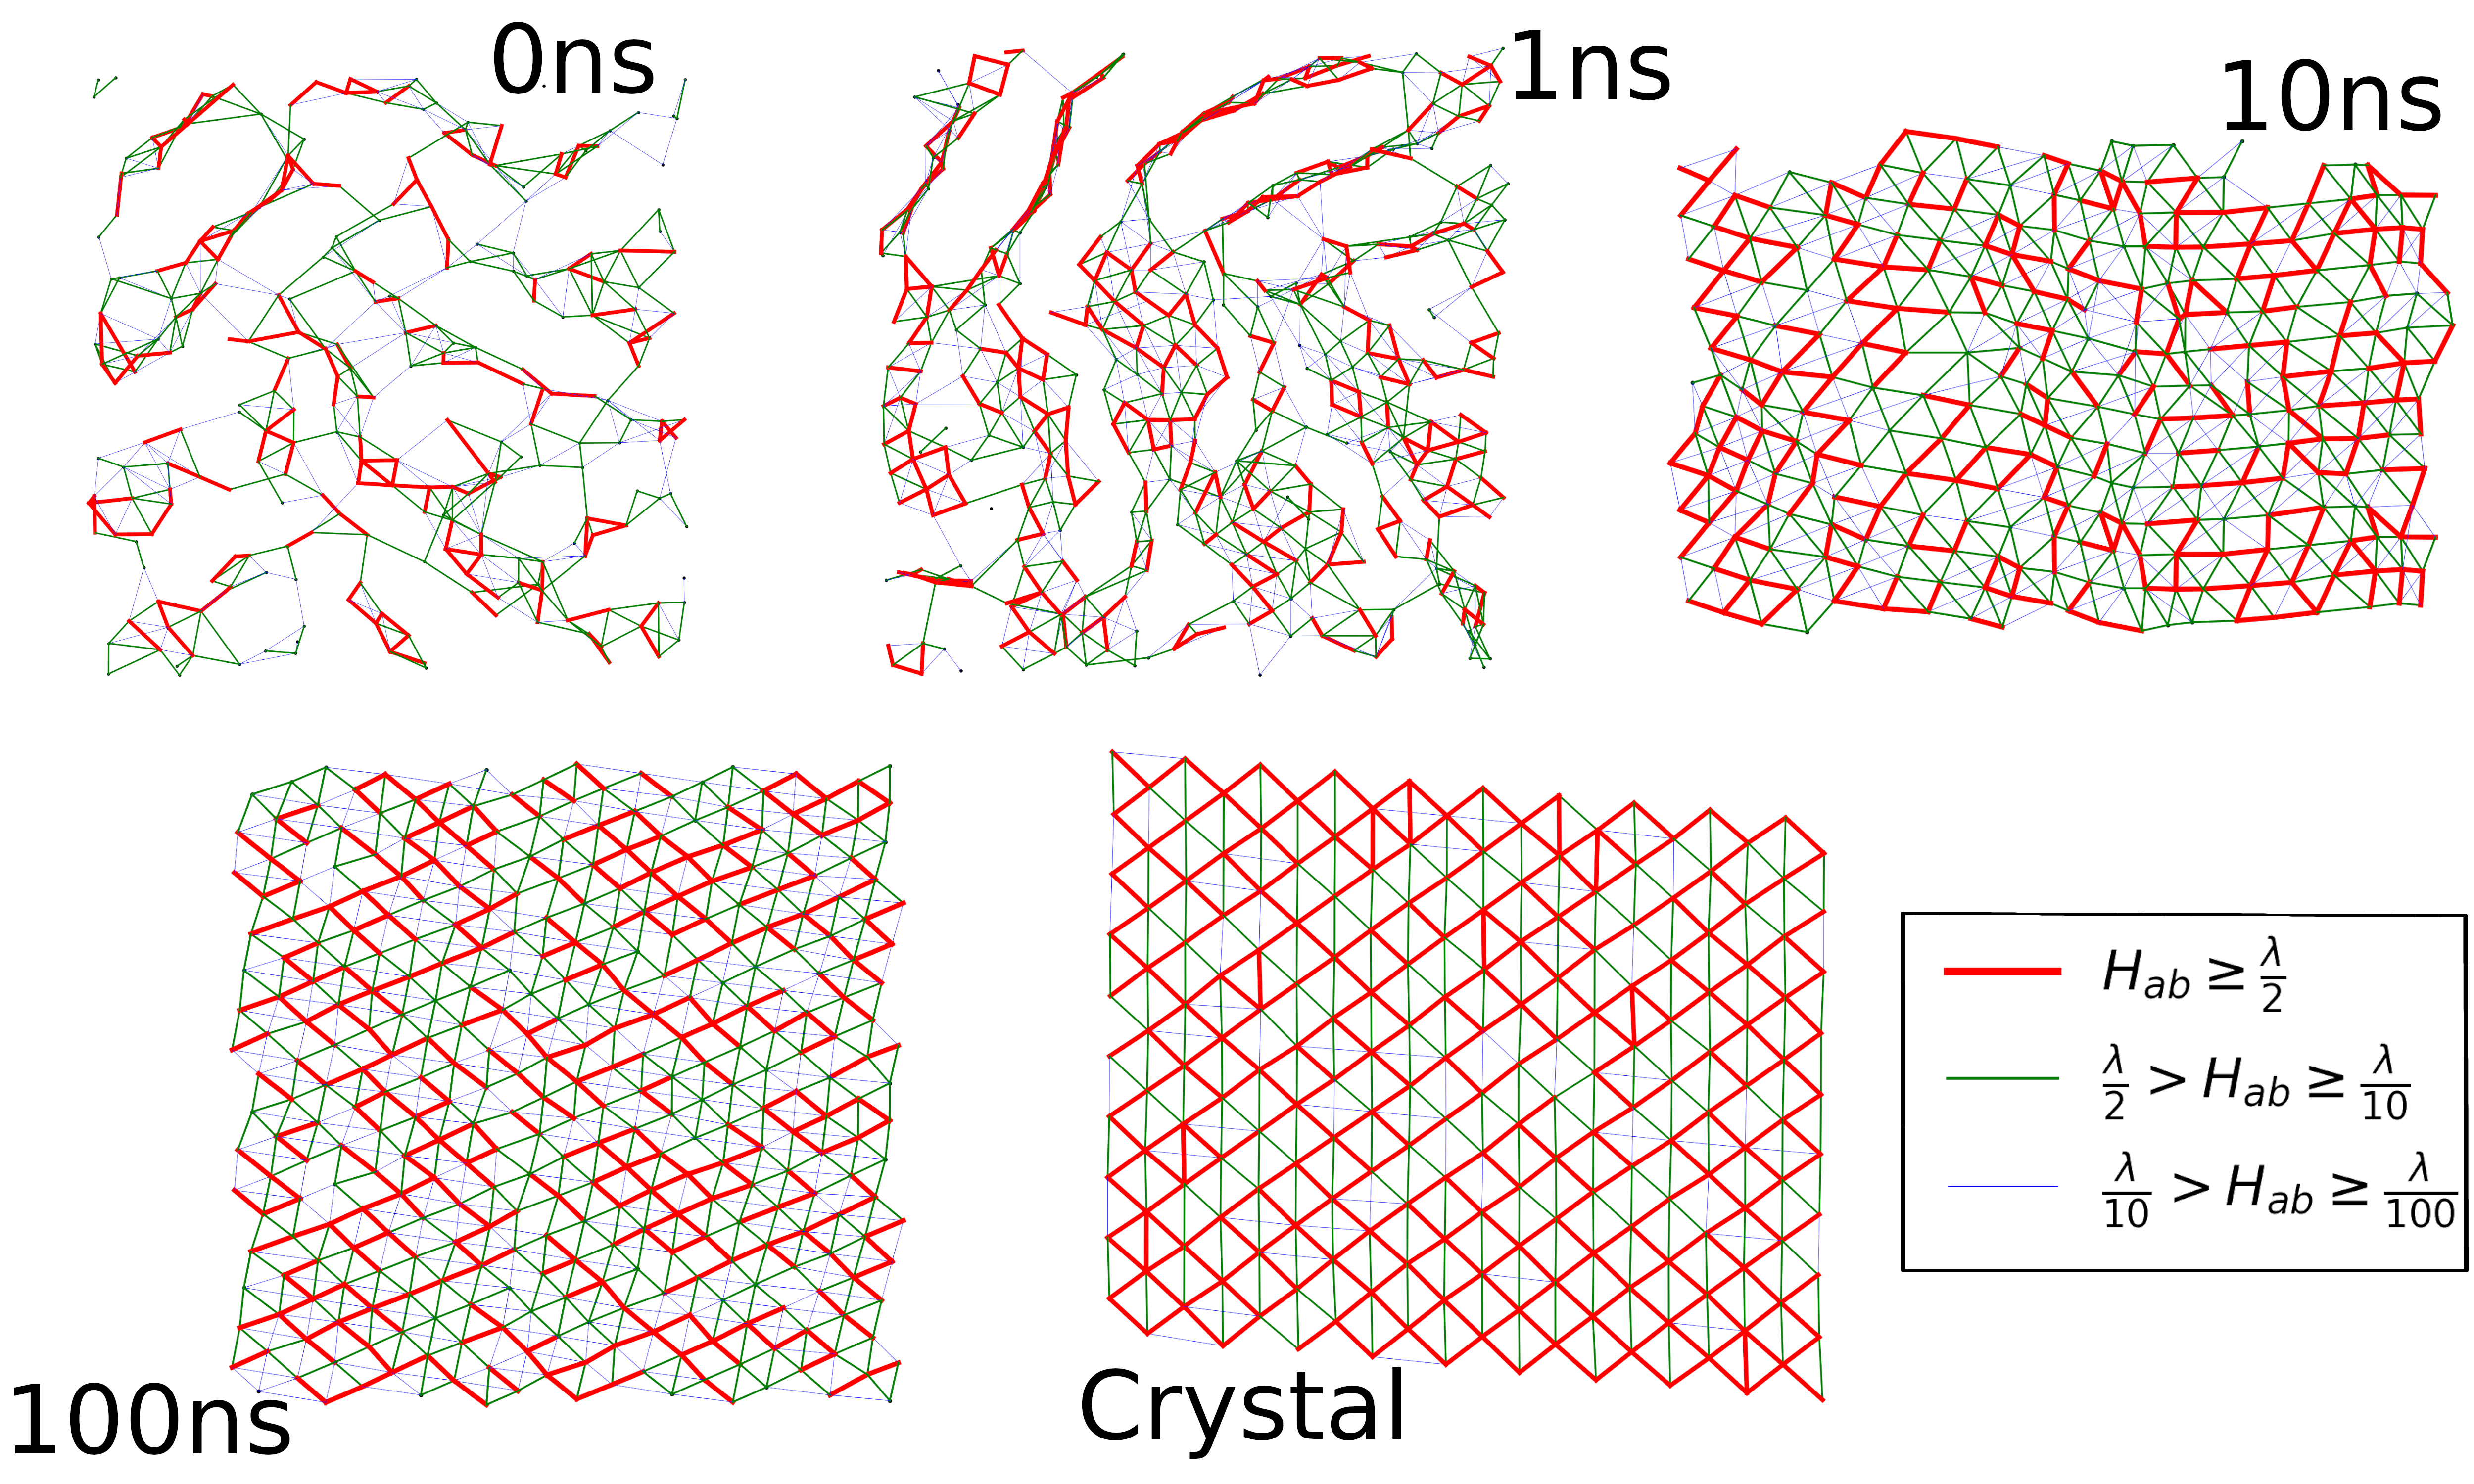
\includegraphics[width=\textwidth]{./img/CouplingPlots/CouplingGraphs_all.png}
	\caption{\label{fig:crystalCouplingGraph}A representative network of electronic coupling that each quenched structure has formed. Each structure is labelled by the quench time (e.g. 0ns, 1ns, 10ns, 100ns) or Crystal for a crystal after a short MD equilibration. Coupling strengths are categorised as high (red), medium (green) and low (blue). The definitions of the categories are given in the legend in the bottom right corner.}
\end{figure}
\noindent In figure \ref{fig:crystalCouplingGraph} the graph of electronic couplings between molecules has been plotted for each of the quenched systems and a crystal system after a short equilibration run with MD. In this figure the centers of mass each molecule is represented by a small black dot and the calculated coupling value with a coloured line (red, green blue). That is, if 2 molecules have a non-negligible coupling between them they would be represented by 2 black dots with either a red, green or blue line connecting them. The couplings were calculated via the analytic overlap method \cite{gajdos_ultrafast_2014} and a pertinent cluster of molecules was selected for each quench time. For the 0ns and 1ns quench times this was simply a slice 1 molecule thick in the z dimension, containing a few hundred molecules. For the 10ns and 100ns quenched structures a reasonable cluster of molecules was chosen after applying a density based clustering algorithm on the superstructure. For the crystal a plane from the crystal was chosen. All panes in figure \ref{fig:crystalCouplingGraph} show the coupling of the selected system from an angle perpendicular to the plane of molecules.
\\\\
We can see in the graph of the 0ns quenched structure there is very little order to the coupling network. Only very small fragments of high (red) coupling are formed and each one is connected via weak or medium coupling. We can define a 'high coupling fragment' as any set of molecules which can all be reached from any member of the set via an unbroken path of high coupling. The mean size of these high coupling fragments in the 0ns structure is 4.1 molecules and there are 503 of them. In this structure we would expect to see a localised polaron (over a $\sim$ 3 molecules) and low mobilities due to the lack of conductive channels in the structure. The mean size of fragments increases and the number of fragments decreases as we increase the quenching time as shown in table \ref{tab:cluster_sizes}.
\\
\begin{table}[ht]
	\begin{tabular}{cccc}
		\textbf{Quench Time} [ns] & \textbf{Mean Fragment Size} & \textbf{Fragment Size Std Dev} & \textbf{Num Fragments} \\
		\hline &&&\\
		0 & 4.2 & 3.8 & 503 \\
		1 & 4.5 & 5.0 & 493 \\
		10 & 6.5 & 9.3 & 373 \\
		100 & 8.7 & 16.2 & 292 \\
		\hline &&&\\
	\end{tabular}
	\caption{\label{tab:cluster_sizes}The change in the number of high coupling fragments, and the mean and standard deviation of their size, found in each structure as the quenching time was varied.}
\end{table}
\\
We can see in table \ref{tab:cluster_sizes} that as the quenching time increases, the size of the highly coupled fragments (how many molecules are connected) increases and fewer of them are formed. The standard deviation also increases, showing in the 0ns structure the fragments are all very small. As the quench time is increased, smaller fragments still appear but much larger ones now form. These larger fragments can act as regions of high conductivity allowing much larger mobilities to be achieved than in the shorter quenching times.

\section{Surface Hopping Methodology}
Several experimental as well as computational studies have indicated that charge transport in crystalline molecular OS falls into a difficult regime where the charge is neither fully delocalised over the bulk material nor completely localised on a single molecule, as had often been assumed.\cite{Vehoff2010,Deng2004,Kwiatkowski2009,Athanasopoulos2007,Vehoff2010_2,Kordt2016,Zhang2019} It has recently been shown, using advanced quantum dynamical simulations, that charge carriers in single-crystalline OS form ``flickering polarons", objects that are half-way between waves and particles\cite{FlickPolarons,Giannini2019,Ziogos20}. It was found they are delocalised over up to 10-20 in the most conductive crystals and constantly change their shape and extension under the influence of the thermal motion of the atoms (crystal vibrations).  Taking the example of bulk crystalline pentacene, it was found that the excess hole is typically delocalised over 17 molecules, in excellent agreement with experimental estimates from electron spin resonance data (17 molecules) The delocalisation of the polaron and mobility are limited by the thermal fluctuations of electronic coupling (off-diagonal electron-phonon coupling) and site energy. This picture of charge transport, obtained by numerically solving the time-dependent electronic Schroedinger equation coupled to nuclear motion, resembles closely, and gives support to, the transport scenario predicted by the recently established transient localisation theory (TLT).\cite{Nematiaram2019,PhysRevB.83.081202}. However, this makes simulating the charge carrier particularly difficult as the 2 standard techniques (hopping and band theories) breakdown in this regime. Further, TLT is inapplicable to systems with high levels of disorder. For this reason, fragment orbital surface hopping (FOB-SH) was used to simulate the motion of the excess charge carrier in each of the samples and hole-mobilities and inverse participation ratios (IPR) were calculated.

\subsection{Surface Hopping Setup}
The surface hopping simulations require a swarm of hundreds of independent trajectories ($\sim$500), each with slightly different geometries to fully sample phase space. To create these trajectories initial positions and velocities were sampled every 1ps from a classical MD simulation (carried out under NVT). In order to initialise the (electron-hole) wavefunction, for each trajectory, the Hamiltonian was calculated. This was then used to find an adiabatic state within 3K$_{B}$T of the ground state energy that was relatively close to the center of the simulated system. The details of this procedure are given in appendix \ref{ap:AdiabaticSelector}. This initialisation of the wavefunction in a low lying adiabatic state allowed for quick convergence of the mean-squared displacement of the charge carrier. Other parameters, such as the method chosen for correcting for over-coherence, trivial crossings and spurious transfer were taken from previous surface hopping simulations carried out by other members of the Blumberger group. The code at the time did not support the calculation of electrostatic interactions. So, in order to maintain the structure from the melt-quench simulations, center of mass restraints were used. These are shown in appendix \ref{ap:restraints}. Finally, the full system for each of the 4 quench times was very large (3,000 mol). So, to sample the mobility at various points within the superstructure the full system was divided into smaller subsystems.The procedure for dividing the superstructure was different for each quench time and full details are given in appendix \ref{ap:system_divisions}. In the 0ns and 1ns quenched runs the full system was divided into 6 roughly even slabs. This was because these structures had very little order and the charge transport was expected to be isotropic. In the 10ns and 100ns quenched systems, a DBCAN-like algorithm \cite{DBSCAN} was used to cluster molecules (by mass-density). These clusters were then used as active regions within the surface hopping code.

\subsection{Inverse Participation Ratio}
The inverse participation ratio (IPR) gives a measure of spread of the polaron. A value of 1 would mean the polaron is localised on a single molecule, a completely delocalised polaron would have a value of $N_{mol}$ where $N_{mol}$ is the number of molecules in the system. The formula used in its calculation is given below in equation \eqref{eq:IPR}:
\begin{equation}
  IPR(t) = \frac{1}{N_{\text{traj}}} \sum_{n=1}^{N_{\text{traj}}} \frac{1}{\sum_{i}^{N_{\text{mol}}} \left| u_{i}^{n}(t) \right|^4}
  \label{eq:IPR}
\end{equation}
Where $N_{\text{traji (mol)}}$ represents the number of trajectory (molecules) and $u_{i}^{n}(t)$ is the diabatic expansion coefficient at time $t$, on replica $n$ and molecule $i$. 
\\\\
The IPR is an important quantity as the level of delocalisation of the wavefunction is positively correlated with its mobility. That is, molecular systems that have a large delocalisation of the charge carrier tend to have larger mobilities. It is also useful in determining if the system has reached equilibrium, as in equilibrium the IPR tends to converge to a constant value.

\subsection{Hole Mobilities}
\label{sect:mobilities}
A full discussion of the calculation of the charge carrier mobility can be found in various papers \cite{Carof17FSSH,Giannini2018Crossover,Giannini2019}. It is calculated from the Einstein diffusion constant, $D$, which in turn is calculated from the change in the mean squared displacement (MSD) of the charge carrier. The MSD is calculated via equation \eqref{eq:MSD} below
\begin{eqnarray}
  \label{eq:MSD_Exact}
  MSD_{ab}(t) &= \frac{1}{N_{\text{traj}}} \sum_{n=1}^{N_{\text{traj}}} \left\langle \Psi^{n}(t) | (\mathbf{R} - \mathbf{R}_{0})^2 | \Psi^{n}(t) \right\rangle \\
  &\approx \frac{1}{N_{\text{traj}}} \sum_{n=1}^{N_{\text{traj}}} \left(\frac{1}{\sum_{i}^{N_{\text{mol}}}} \left| u^{n}_{i}(t) \right|^2 (\mathbf{R}_{i}^{n}(t))^2 \right)
  \label{eq:MSD}
\end{eqnarray}
Where $\Psi^{n}$ is the wavefunction for trajectory $n$, $\mathbf{R}$ is the position coordinate and $\mathbf{R}_{0}$ is the position coordinate at time $t=0$. $\mathbf{R}_{i}^{n}(t)$ is the time-dependent position of the center of mass of molecule $i$ on trajectory $n$. Equation \eqref{eq:MSD_Exact} is the exact quantum mechanical equation for the MSD, equation \eqref{eq:MSD} is the equation that is used to calculate the MSD from the surface hopping output. The quantity is in general a 3x3 matrix and the values $a$ and $b$ are indices indexing each of the 3 Cartesian dimensions.
\\\\
After a small equilibration the MSD increases linearly. This is indicative of Einstein diffusion and the coefficient can be calculated, in this linear regime, as in equation \eqref{eq:DiffConst} below:
\begin{equation}
  D_{ab} = \frac{1}{2} \lim_{t \rightarrow \infty} \frac{d}{dt}MSD_{ab}(t)
  \label{eq:DiffConst}
\end{equation}
In order to calculate the time-derivative of the MSD, a line of best-fit is fitted to the MSD vs simulation time and the gradient is calculated. This is then used in the calculation of the mobility in equation \eqref{eq:mobility} below.
\begin{equation}
	\mu_{ab} = \frac{e D_{ab}}{k_{B} T}
	\label{eq:mobility}
\end{equation}
Where $k_{B}$ is the Boltzmann constant, $e$ the elementary charge and $T$ is the temperature. The charge mobility is a quantity that can be calculated in experimental studies, so is an important quantity to calculate. It shows how quickly charge can be transported across a system and can be used to calculate other important quantities such as drift velocity ($v_{d} = \mu E$) or conductivity ($\sigma \propto \mu N_{carrier}$).
\subsection{Surface Hopping Results}
\begin{figure}[htp] 
  \includegraphics[width=\textwidth]{./img/DifferentQuenchTimes/mobilities.png}
  \caption{\label{fig:mobilities}IPR and hole mobility vs crystallinity as defined in equation \eqref{eq:crystallinity}. Filled in markers represent experimental values and hollow markers represent data from computational simulations. Blue markers represent mobilities and green markers represent IPR values. Large hollow circles show the mean of results from simulations on various regions within the superstructure (small hollow circles).}
\end{figure}
\subsubsection{Quantum Localisation}
The IPR is plotted, along with the hole mobility, in figure \ref{fig:mobilities} for the amorphous, nanocrystalline and single crystalline samples. It is clearly visible that the delocalisation of the carrier wavefunction, defined in terms of the inverse participation ratio (IPR, Eq.~\ref{ipr}), increases with increasing crystallinity, reflecting the trend seen in the electronic coupling maps. In the amorphous sample, the static disorder of electronic coupling results in the wavefunction localising, on average, over just 2-3 molecules. At 30\% and 60\% crystallinity, the high concentration of defects restricts wavefunction delocalisation over 5-6 molecules, whereas at 80\% we observe a marked increase to 10 molecules, which is still some way off from the value for the single crystal, 17 molecules.  At this point we also see for the first time a clear spatial anisotropy of the charge carrier wavefunction extending more strongly along the T1 high coupling direction in the pentacene crystal (diagonal direction in Figure \ref{fig:crystallinity}). Remarkably, we notice a good correlation between the IPR and the cluster size in the electronic coupling map (Table \ref{tab:cluster_sizes}) suggesting that carrier delocalisation is limited by static disorder of electronic coupling. This correlation is lost for the single crystal because in this case delocalisation is limited by the thermal disorder of electronic couplings (i.e., dynamic or electron-phonon coupling). 
\subsubsection{Hole Mobilities}
Hole mobilities for all samples were obtained as explained in section \ref{sect:mobilities}. For each superstructure multiple active regions were selected to calculate a mobility for. These ``local" charge mobilities can show the impact of structural inhomogeneity of the quenched samples on charge transport. We find that in the disordered samples, especially the one with $\sim$30\% crystallinity, the local charge mobilities and IPR values exhibit a relatively large spread as some regions are more crystalline and thus more conductive than others (Figure \ref{fig:mobilities}, small open circles). In the structurally more homogenous sample with 80\% crystallinity, the variation in local mobility becomes almost negligible. The average of the local charge mobilities and IPRs correlate well with the crystallinity of the sample (Figure \ref{fig:mobilities}, large circles). Over the last 20 years a large number of experimental hole mobilities have been reported for pentacene thin films and crystals from organic field effect transistor (OFET) measurements. Yet, there are several issues to consider when comparing our calculations to these measurements. In OFETs charge transport is typically probed on the micrometer scale over macroscropic time scales, whereas present calculations are carried out for nanoscale samples over short times (ps-ns). Moreover, OFET mobilities have been shown to be very sensitive to many details of the preparation method including, e.g., the gate dielectric used, the surface roughness, deposition rate and temperature etc. This can be seen in the very large spread of experimental mobilities  for amorphous pentacene (figure \ref{fig:mobilities}, solid pentagons). My calculated value of hole mobility, of 0.14 cm$^2$ V$^{-1}$ s$^{-1}$, fits towards to upper end of this spread. It is suspected that the inclusion of electrostatic interactions may reduce this further. This may be due to increased trapping of the polaron from larger levels of energetic disorder (larger site energy differences in the language of FOB-SH). That is the inclusion of electrostatics is thought to increase the energy penalty from transitioning from an initial state with $N_{init}$ states charged to the final state with $N_{final}$ states charged. It is not thought that these extra interactions would affect the more crystalline systems, as contrary to the amorphous case, each molecule feels a very similar electrostatic potential due to the very ordered nature of the structure. A fuller discussion of the role of electrostatics can be seen in Martinelli et al \cite{ESEffectOnMob}.
\\\\
Notwithstanding the above caveats, the correlation between experiment and computed FOB-SH mobilities is rather good, which supports the mechanistic picture that our simulations have revealed. The simulated results have been compared to experimental values for the fully amorphous and fully crystalline samples. For the fully crystalline sample the agreement to experiment is very good, our simulations produced a value of 10.3 cm$^2$ V$^{-1}$ s$^{-1}$ whereas experimental studies have reported values ranging from 5-10.5 cm$^2$ V$^{-1}$ s$^{-1}$. Again the value reported in this work sits at the upper end of the experimentally reported values for reasons discussed previously.

\section{Conclusions}
In this chapter, I have presented a molecular dynamics method for tuning the crystallinity of a pentacene sample based on melting and subsequently quenching the sample over various timescales. I have shown, as was expected, that longer quench times lead to more ordered structures and discussed the mechanism leading to this. That is, in longer quench times the few crystal fragments that begin to seed have a longer time to grow before their growth is impeded by neighbouring crystal fragments. I have displayed various macroscopic properties that confirm that the longer quench times do indeed show more order, including mass-density, angular distribution and the radial distribution function. Further, I have presented networks of electronic coupling within each of the quenched systems, that can be used to get a qualitative feel for the electronic transport properties without expensive quantum dynamics simulations.
\\\\
In calculating quantitative values for hole mobilities to compare to experimental values, I have shown that it is now possible to use explicit quantum dynamical calculations to simulate charge carrier transport in large, realistic samples of disordered organic semiconductors. My results are in remarkably good agreement with those available from experiment and provide a molecular-scale picture of the Nature of the charge carrier and the transport mechanism as a function of the crystallinity of the system. The notion that charge carrier transport in disordered systems occurs via small polaron hopping is shown to be a reasonably good approximation only for fully amorphous systems - for semi-crystalline and crystalline samples significant charge carrier delocalization occurs mandating the use of more advanced transport simulations, e.g.  the FOB-SH method used here. In general, there is a good correlation between crystallinity, carrier delocalization and mobility.  Interestingly, we find that even relatively small amounts of structural disorder can lead to a significant drop in charge carrier delocalization and hole mobility compared to the single crystal. This is an important consideration when comparing charge carrier mobilities in simulated organic systems, usually perfectly crystalline, with those of experiment, where it is difficult to prepare highly pure crystals devoid of defects. This approach is generally applicable to any molecular organic semiconductor and may be used for identifying new disordered materials with high charge mobility. 
\\\\
Finally, this study has served to highlight a potential drawback in the FOB-SH methodology as it currently stands. That is, the lack of electrostatic interactions within the simulations. These have not been implemented previously as the group's work was focussed on perfect crystals, where electrostatic interactions are not expected to affect the final result. However, in the more disordered systems this approximation may be a step too far. In the final chapter of this thesis, I will present my implementation of electrostatics within the surface hopping and a possible alternative to expensive Ewald summation.



